\chapter{持续学习}

\section{SSIAT：从发现分布偏移，到适应分布偏移}

在《DML：为什么模型的置信度不等于模型对世界的认识程度？》《DPM：视觉语言模型如何认识未知？——从语义识别到分布认知》《ASL：既然方向很重要，能不能在训练阶段塑造更好的角度空间？》《OSPCoOp: 从识别未知类别，到识别模型判断中的错误依据》系列中，我们系统思考了 AI 模型（比如 Transformer、CLIP）如何发现训练分布之外的数据，或者说检测分布偏移，也探讨了模型在训练中如何学习特征空间以更好地刻画语义。测试时发现数据较之训练分布有变化之后，模型要适应这种变化——语义上的变化、数据域的变化甚至两者兼而有之。现在，我们先从适应语义变化说起。

语义是什么？简单说就是：数据所表达的内容和含义，而不是数据的外观。例如，在图像识别中，一张猫的照片，不管是黑猫、白猫，还是卡通猫，它表达的语义都是“猫”；一张汽车的照片，不管是在白天、夜晚，还是雨天，它表达的语义都是“汽车”。所以，语义的一种简练的变现形式就是类别标签。AI 模型运行在开放环境中需要持续去学习：今天识别猫狗，明天可以增加之前没见过汽车，后天又增加飞机等新的类别——这就是增量学习。难点是什么？面对未知的新增类别，模型指导语义分布偏移了，但总是难以估计语义到底偏移了多少（Semantic Shift）。对此，我们假设：如果一批新图片在模型更新前后整体向某个方向移动了，那么与它们在旧特征空间中比较接近的旧类别的特征中心也可能受到相似方向的影响。具体步骤上，我们可以在旧模型中提取新图片的特征，在更新后的模型中再次提取同一批图片的特征，然后计算新旧模型之间的特征变化；基于上述假设，再把新图片的特征变化汇总起来，就可以估计每个旧类别的 Semantic Shift，用以更新旧类别原型——这就是 Semantically-Shifted Incremnetal Learning。

模型本身能支持这样的增量式的更新吗？对于 Transformer，更新模型的一种主要方式是参数微调。然而，完整微调需要更新大量参数，训练和存储成本较高。一种比较高效的参数微调方法是适配器微调（Adapter Tuning）：在 Transformer 中插入少量可训练的适配器模块，同时冻结原有预训练参数，从而以较低的参数更新成本实现模型适配。至于其它的参数微调方法，Prompt Tuning 能持续更新共享 Prompt 但旧类别容易遗忘， SSF 能持续更新缩放和平移参数但容易过拟合当前阶段。

\begin{figure}[H]\centering
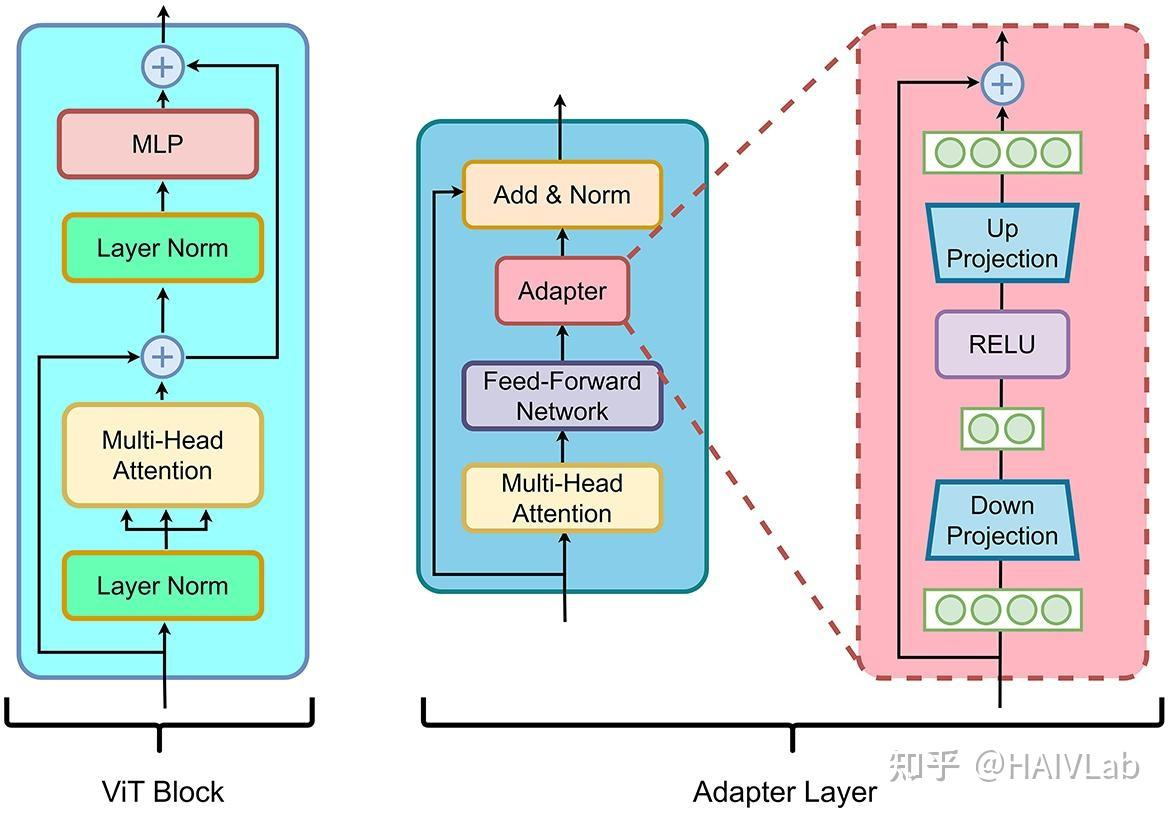
\includegraphics[width=0.82\linewidth,height=0.42\textheight,keepaspectratio]{figures/vit_block.png}
\caption*{Adapter 可以理解成插入 Transformer 的一个小型可训练模块}
\end{figure}

在 Adapter Tuning 这种范式下，Transformer 模型本身支持增量式更新——每当引入新类别样本时，都继续更新同一个 Adapter（而不是为每个新类别都增加一个新的 Adapter）。有鉴于上述我们有估计语义偏移的策略，我们对 Adapter 的更新基本上没有任何限制，所以模型总能识别新类别——新类别和旧类别兼顾到了（Semantically-Shift Incremental Adapter Tuning, SSIAT）：有了更新后的旧类别原型，以及当前阶段新类别的原型，将每个类别的特征分布近似为一个高斯分布 $\mathcal{N}(\mu_c,\Sigma_c)$，然后从每个类别的高斯分布中采样特征，构造一批虚拟特征样本。最后，用这些样本重新训练一个统一分类器，就不需要保存旧类别的原始图片，也能重新平衡新旧类别的分类能力。

\begin{figure}[H]\centering
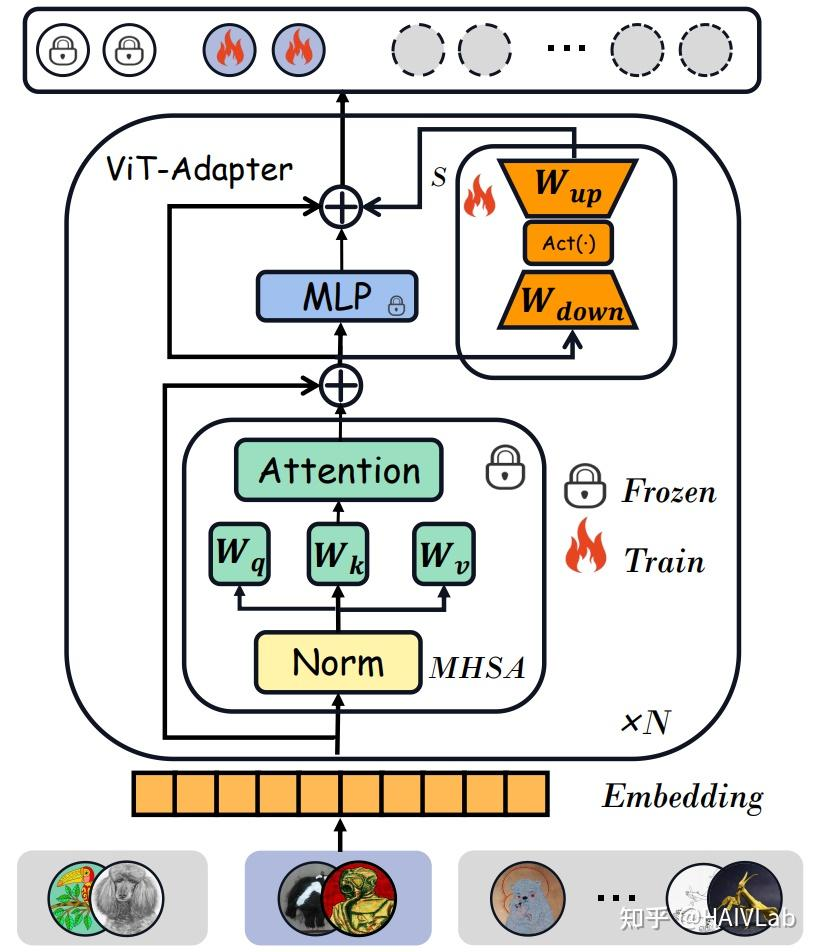
\includegraphics[width=0.82\linewidth,height=0.42\textheight,keepaspectratio]{figures/vit_adapter.png}
\caption*{Adapter 和分类器在每个阶段用新样本增量式样训练更新}
\end{figure}

我们在五个增量学习基准上进行了实验，包括 CIFAR100、CUB200、ImageNet-R、ImageNet-A 等。例如，CIFAR100 上的平均增量准确率：

\begin{table}[H]\centering
\caption*{CIFAR100 平均增量准确率}
\begin{tabular}{ll}\toprule
\textbf{方法} & \textbf{平均准确率} \\ \midrule
SLCA & 94.29\% \\
Adam-Adapter & 91.21\% \\
SSIAT & 94.35\% \\
\bottomrule\end{tabular}
\end{table}

SSIAT 在这个设置下取得了很有竞争力的结果，同时只训练少量 Adapter 参数，不需要保留旧类别的图片。展示了一个可行的设计：预训练模型提供基础表示能力，Adapter 提供持续学习能力，原型更新负责补偿历史特征漂移。

总而言之，SSIAT 认同学习新知识会改变旧知识的表示这一问题的存在——即使保存了旧类别的原型，它们也可能因为特征提取器变化而失，但也主张保护旧知识不等于冻结模型——如果过度限制参数变化，模型就难以学习新类别，所以选择持续更新共享 Adapter，并通过原型语义偏移估计和分类器重训练来弥补旧知识的变化。更全局的看，OOD Detection 和 Continual Learning 不是简单的前后替代关系。

\begin{itemize}
  \item OOD Detection 主要回答：发生了什么变化？输入是否超出了当前模型的已知分布？
  \item Continual Learning 主要回答：出现了新知识后，模型如何学习，同时保留旧知识？
  \item Test-Time Adaptation 主要回答：不改变任务类别定义的情况下，如何适应输入分布
\end{itemize}

的变化？

\paragraph{相关工作}

\begin{itemize}
  \item Yuwen Tan, Qinhao Zhou, Xiang Xiang*, Ke Wang, Yuchuang Wu, Yongbin Li: SemanticallyShiftedIncrementalAdapter-Tuning is AContinualViTransformer. In CVPR, 2024.
\end{itemize}

\section{RAA：持续学习不仅要考虑模型学到了什么，还要考虑模型是如何改变自己的}

\begin{figure}[H]\centering
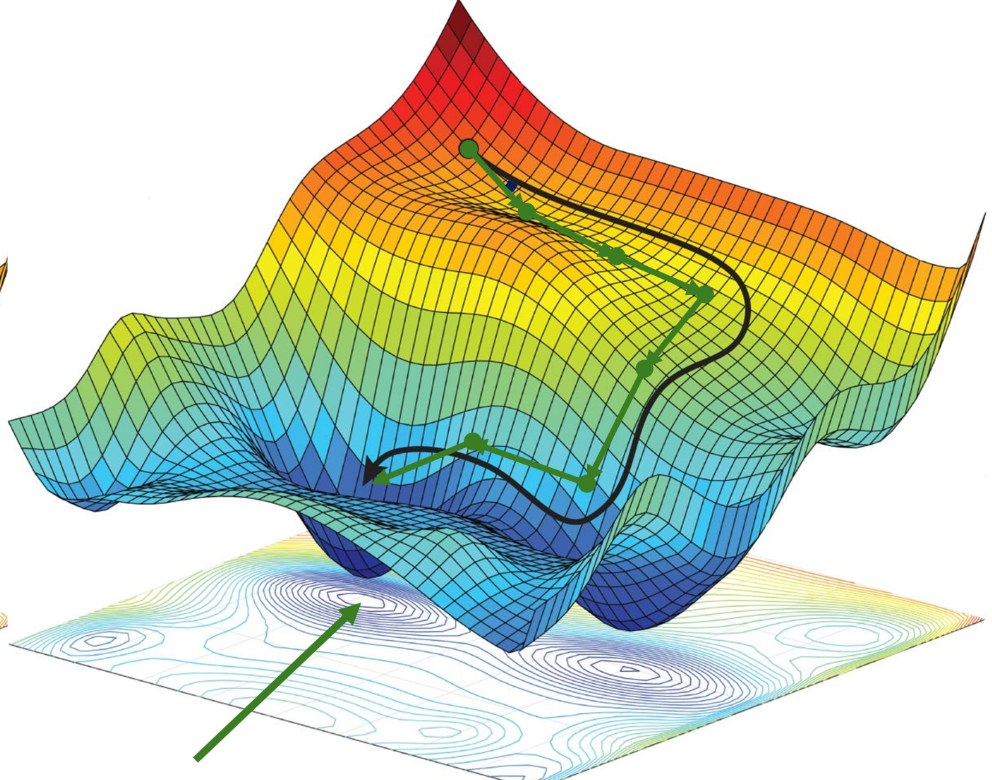
\includegraphics[width=0.82\linewidth,height=0.42\textheight,keepaspectratio]{figures/landscape.jpg}
\end{figure}

在《SSIAT：从发现分布偏移，到适应分布偏移》中，我们关注旧类别的特征表示发生了什么变化——新类别学习导致旧类别在特征空间中的表示发生漂移：通过估计 Semantic Shift，更新旧类别原型，再利用生成的特征样本训练分类器。现在，我们不再主要从特征方面入手，而是从分类器方面关注模型参数更新为什么会造成遗忘——研究 AI 模型的损失函数的 Loss Landscape。

模型最初学习猫和狗，后来不断增加汽车、飞机、鸟类等新类别。假设模型使用 Vision Transformer (ViT)，并像 SSIAT 中方式那样通过 Adapter 微调。每学习一个新阶段，Adapter的参数都会更新。问题在于：参数更新幅度相同，并不意味着对旧知识的影响相同。有些模型的参数稍微变化，旧类别的识别能力就大幅下降；另一些模型即使参数发生类似变化，旧类别的性能仍然比较稳定。这种问题，在机器学习里可以关联到一个概念：Loss Landscape（损失景观）的平坦程度。

\begin{figure}[H]\centering
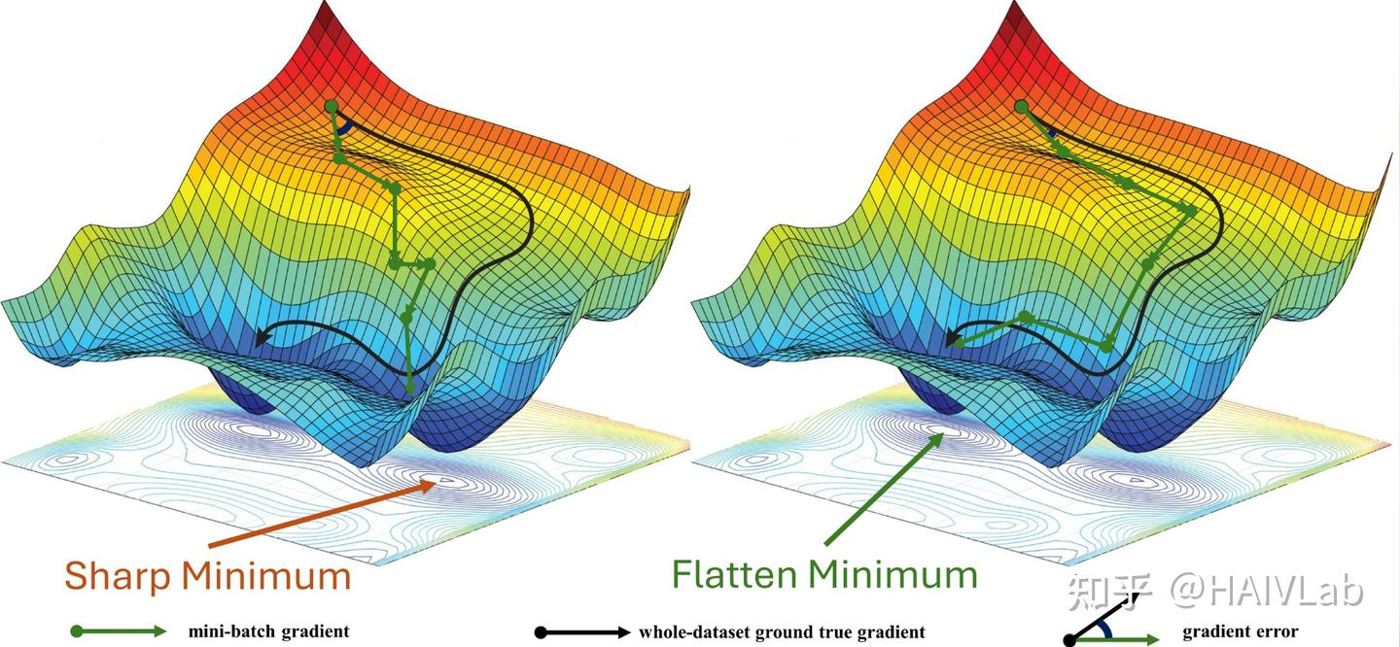
\includegraphics[width=0.82\linewidth,height=0.42\textheight,keepaspectratio]{figures/sharpflat.png}
\caption*{如果模型处在一个尖锐的低谷：参数稍微移动，Loss 就迅速增大。如果模型处在一个平坦的低谷：参数在附近发生一定变化，Loss 仍然比较小}
\end{figure}

学习新类别时，模型参数不可避免地要改变。如果原来的模型处于一个平坦区域，那么参数更新后，旧类别的 Loss 更有可能保持较小。那是不是 Loss Landscape 越平坦，模型就越稳定、遗忘也越少呢？

\begin{figure}[H]\centering
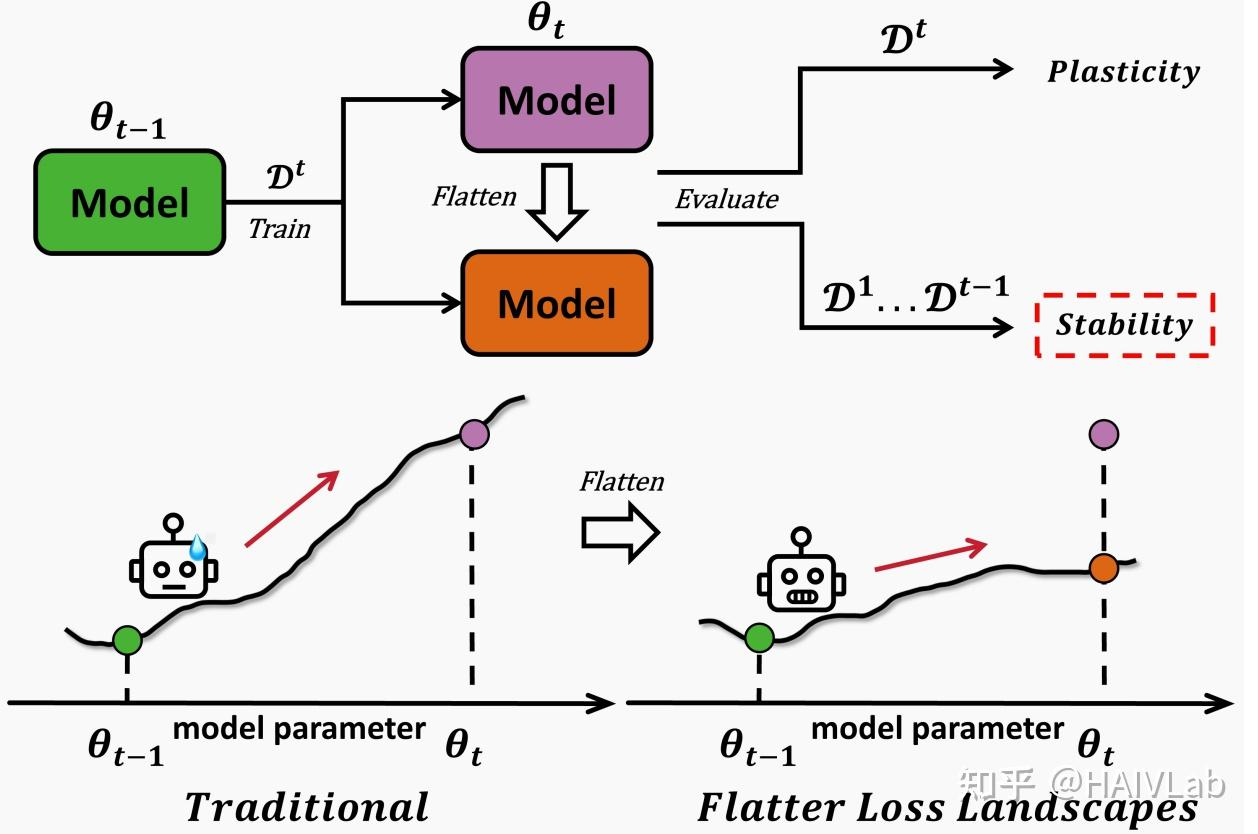
\includegraphics[width=0.82\linewidth,height=0.42\textheight,keepaspectratio]{figures/flatter.png}
\caption*{Adapter Tuning ViT 增量学习过程中确实发现：如果后续阶段的损失函数更平坦，模型训练更能保持在小的损失上}
\end{figure}

既然希望模型在参数变化时仍然保持较小 Loss，一个直接的想法是：不要只训练一个Adapter，而是训练多个 Adapter。如果它们都插入同一个预训练的 ViT 中但各自独立优化，那么模型就不再只适应一个参数点，而是有机会在多个参数配置下保持较好的性能。但是，多个独立 Adapter 只是多个离散的参数点，并不意味着它们之间的参数组合也能保持低Loss，甚至模型未必还能正常工作。

怎么组合多个 Adapter？随机组合 Adapter（Random Amalgamation of Adapters, RAA）！不只让多个 Adapter 各自表现良好，还要让它们随机组合之后，模型依然能够正常工作。假设有两个 Adapter：

\[
A,\quad B
\]

训练时随机生成组合权重：

\[
\omega A+(1-\omega)B
\]

每次训练随机采样 $\omega$，例如：

\begin{itemize}
  \item 第一次：0.8A + 0.2B；
  \item 第二次：0.3A + 0.7B；
  \item 第三次：0.5A + 0.5B。
\end{itemize}

模型每次都使用随机组合后的 Adapter 进行训练。因此，它必须适应各种不同的参数组合，而不是只适应 A 或 B 两个独立的配置。于是，模型被迫在更广泛、更加连续的参数空间中维持较低的 Loss。并且是在训练过程中随机组合 Adapter 参数，最终仍然得到一个可以部署的模型。

但是损失函数只是训练分类器的一方面，另一方面是优化求解。即使参数空间已经比较平坦，优化算法仍然可能沿着不理想的方向更新参数。既然 Loss Lanscape 已经尽量平坦了，求解过程要对 Landscape 的 Sharpness 有所认知——不同于普通训练只关心当前参数位置的Loss 是否足够小，要进一步考虑如果参数稍微受到扰动，Loss 会不会突然变得很高？所以在优化上，倾向于寻找附近一片区域内都保持较低 Loss 的参数，而不只是找到一个孤立的低点——Sharpness-Aware Minimization（SAM）。并针对参数增量学习的特点，估计模型参数更新方向与损失尖锐方向之间的关系，再通过一个调节系数控制更新幅度：如果当前参数更新方向容易进入 Loss 快速上升的区域，就降低这次更新的幅度；如果更新方向相对安全，就允许正常更新。即不是简单地让学习率变小，而是根据参数更新方向与尖锐方向的关系，动态调节更新。

实验方面，使用 ViT-B/16，在 ImageNet-21K 预训练模型，覆盖五个主要数据集（ImageNetA、ImageNet-R、CUB200、Stanford Cars 、CIFAR100），比较的方法既有 Adapter、Prompt方法，也有 RanPAC、SLCA、SSIAT 等增量学习方法。

\begin{table}[H]\centering
\caption*{五个数据集平均结果}
\begin{tabular}{lll}\toprule
\textbf{方法} & \textbf{最终准确率 ALast} & \textbf{平均准确率 AAvg} \\ \midrule
RanPAC & 78.24\% & 83.82\% \\
SLCA & 76.80\% & 82.27\% \\
SSIAT & 76.43\% & 81.89\% \\
RAA（Ours） & 79.73\% & 84.22\% \\
\bottomrule\end{tabular}
\end{table}

这里的 ALast 是完成所有增量阶段后的准确率，AAvg 是各阶段准确率的平均值。RAA 在五个数据集的平均结果上取得了最好的表现。

尤其值得注意的是 Stanford Cars：

\begin{itemize}
  \item RAA：72.39\%
  \item RanPAC：68.89\%
  \item 第二名之外的领先幅度约为 3.5 个百分点。
\end{itemize}

ImageNet-A 上，RAA 最终准确率为 64.06\%，也超过 SSIAT 的 62.43\%。

总而言之，RAA 这个工作通过随机组合 Adapter 和 SAM+，提高模型对参数变化的稳定性：RAA 方法本身让不同 Adapter 的随机组合都具有较好的性能；SAM 让参数更新尽量避开损失快速上升的方向；两者结合，既扩大了低 Loss 区域，也让优化过程更稳定。RAA 的价值不在于无限增加参数，而在于更有效地利用有限参数。

不同于 SSIAT 从表示空间入手修正旧类别的语义漂移，RAA 从参数空间入手降低增量更新对旧知识的破坏。传统增量学习主要关注新旧类别的准确率、遗忘程度，以及如何保留旧知识。 RAA 则进一步把视角转向模型参数空间：如果模型在一个平坦的低损失区域内学习，那么它对后续参数更新就可能更加稳定。凭借这个工作，我们把我们的持续学习研究关注点从特征空间扩展到了参数空间，并进一步思考能否同时维护表示空间的稳定性和参数空间的稳定性。

\paragraph{相关工作}

\begin{itemize}
  \item Yao Deng, Xiang Xiang*, Jiaqi Gui. Random Amalgamation of Adapters for Flatter Loss Landscape: TowardsClass-Incremental Learningwith Better Stability. In AAAI, 2026 (Oral).
\end{itemize}

\section{C2FSCIL \& Knowe：从类别增量学习走向语义细化}

\begin{figure}[H]\centering
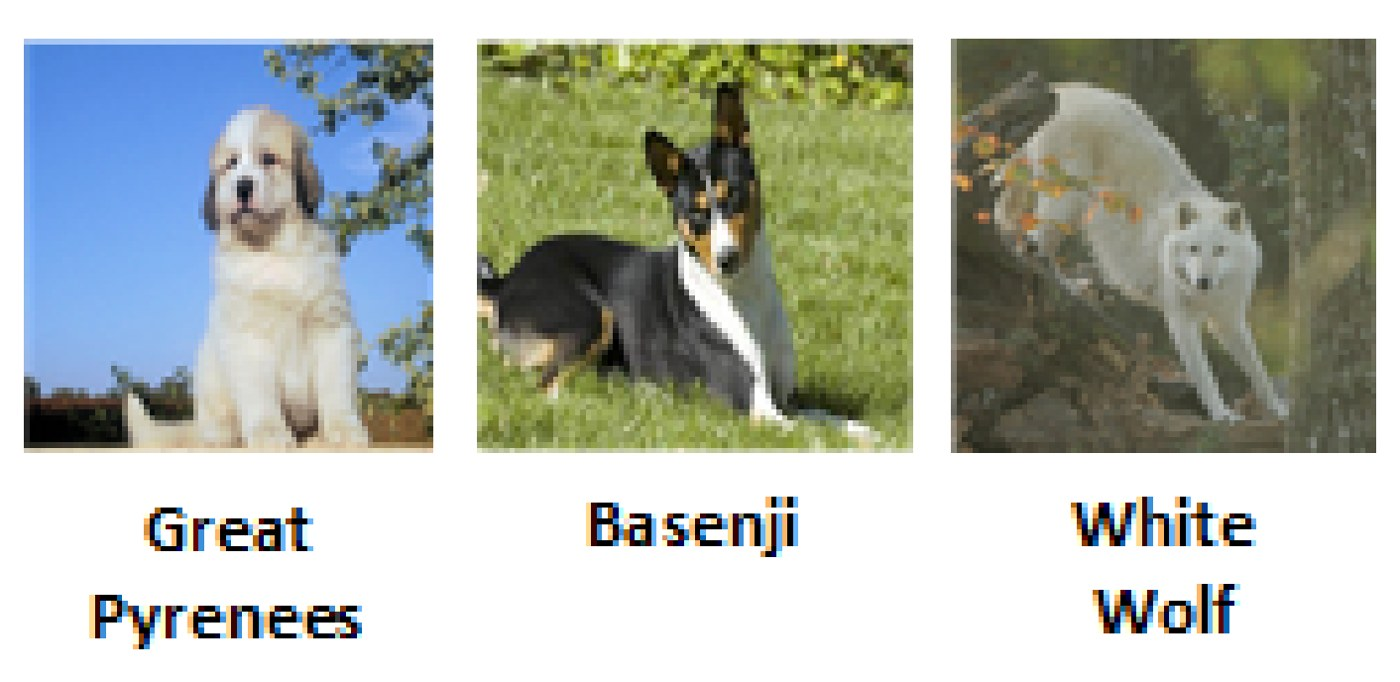
\includegraphics[width=0.82\linewidth,height=0.42\textheight,keepaspectratio]{figures/dogs.jpg}
\end{figure}

在《SSIAT：从发现分布偏移，到适应分布偏移》和《RAA：持续学习不仅要考虑模型学到了什么，还要考虑模型是如何改变自己的》《EHS：预留类别扩展的特征空间》中，我们分别从特征表示的语义偏移和模型参数更新的稳定性出发，探讨了持续学习过程中如何适应变化、减少遗忘。特别实在《EHS：预留类别扩展的特征空间》中，我们已经在思考未来出现新类别时，特征空间如何容纳它们。但是，语义变化并不总是表现为已有类别的特征分布发生偏移。在开放世界中，我们对事物的认识也可能不断深化：最初，模型只能识别一个粗粒度类别；随着新数据和新知识的到来，它需要进一步区分这个类别下更具体的子类别。例如，模型最初只能识别“狗”，后来需要逐步学会区分哈士奇、金毛和柯基。这时，问题不再只是如何适应特征分布的变化，而是如何适应类别语义结构从粗到细的演进。如何让模型在保留已有知识的同时，不断细化对世界的认识？这引出了从类别增量学习走向语义细化的问题——模型必须在已有粗粒度知识的基础上，逐步学习新的细粒度类别，同时保留原来对粗粒度类别的识别能力。这就是 Coarse-to-Fine Few-Shot Class-Incremental Learning，简称 C2FSCIL。

它和普通类别增量学习有一个重要区别：普通类别增量学习通常是在已有类别之外增加新的类别；而这里的新类别是已有类别的进一步细分。不用任何特别处置的话，就是每次拿到新的细粒度样本后直接微调模型。例如，模型最初已经知道某张图片属于“狗”。现在拿到几张巴仙吉犬的图片，用“巴仙吉犬”这个新标签继续训练。这会出现问题：模型为了适应新的细粒度标签，会调整原来的特征表示和分类器；而训练过程中只有当前新类别的少量样本，原来的粗粒度训练数据又不能拿回来，因此微调下去模型很容易出现灾难性遗忘掉原先的知识。

\begin{figure}[H]\centering
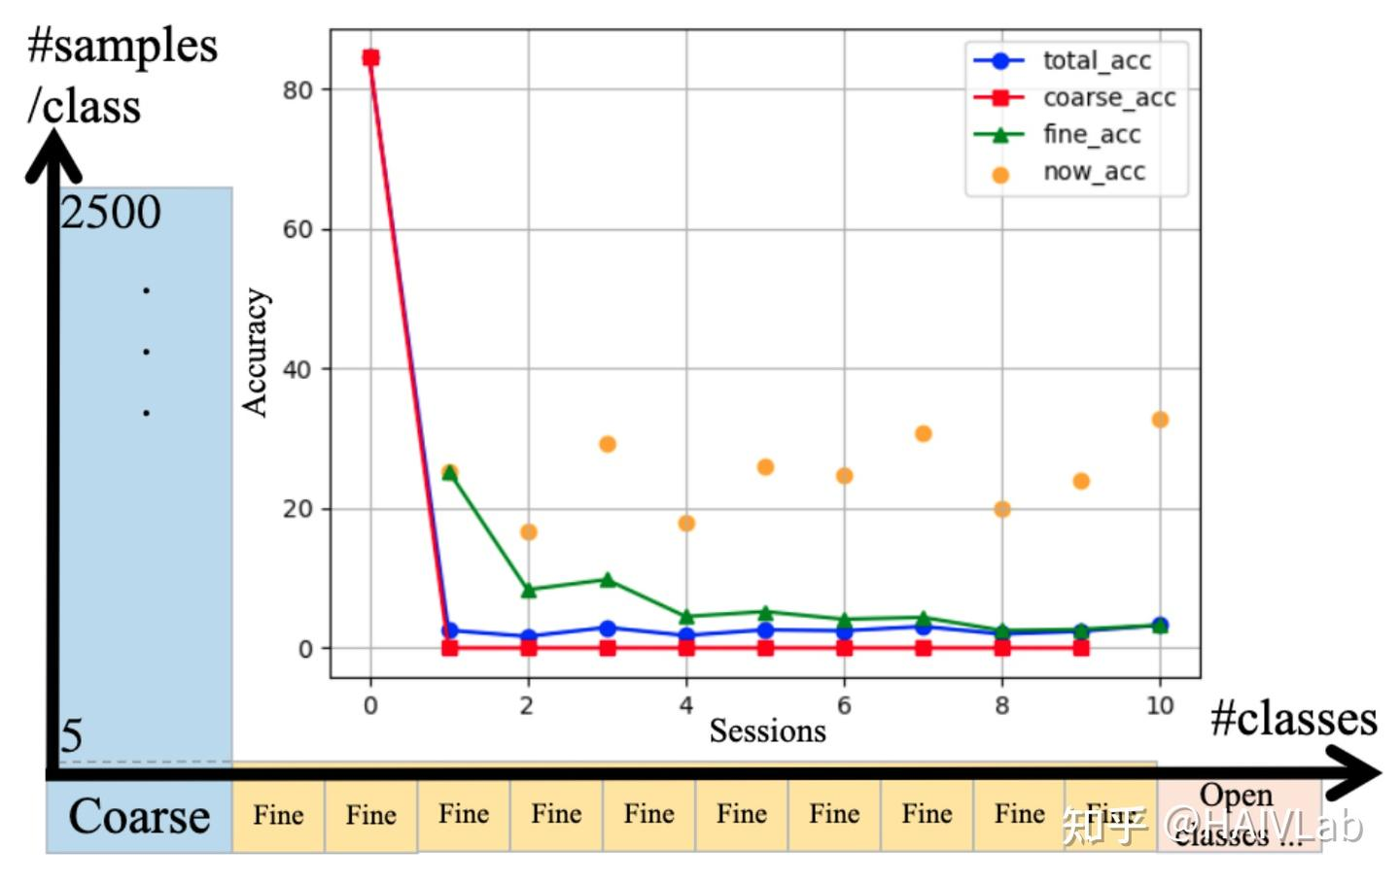
\includegraphics[width=0.82\linewidth,height=0.42\textheight,keepaspectratio]{figures/curve.png}
\caption*{在连续学习细粒度类别的过程中，模型原来对粗粒度类别的识别能力迅速下降那么，对类别语义从粗到细的变化，应该如何让模型具备适应能力？一个关键问题在于：模型在最初训练时，是否考虑过未来的语义细化？如果模型在初始阶段只针对粗粒度类别进行优化，那么它学到的特征表示可能只需要区分不同的粗粒度类别，而不必保留同一粗粒度类别内部的细粒度差异。例如，当模型只需要识别“狗”这一类别时，它没有充分的训练动机去区分哈士奇、金毛和柯基。等到未来需要识别这些子类别时，再试图通过少量增量样本让模型建立新的细粒度判别能力，就可能面临很大的困难：原有的特征表示未必保留了足够的区分信息，而大幅调整模型又可能破坏已经学到的知识。因此，语义细化不应该完全被视为增量阶段才需要解决的问题。如果能够在模型最初训练时，就考虑到未来类别可能从粗粒度向细粒度演进，那么我们就有机会提前塑造更适合细粒度学习的特征表示。所以，我们在基础训练阶段需要利用粗粒度监督，为未来的细粒度学习提前准备特征表示。Knowe 的做法是：}
\end{figure}

第一步：先利用粗粒度标签学习一个具有泛化能力的特征空间通过对比学习，让同一粗粒度类别内部的图像形成有组织的特征表示，同时利用分类损失区分不同粗粒度类别。对比学习不只是把同类样本拉近，还特别关注同一粗粒度类别内部的不同样本之间的差异，以保留未来细粒度分类可能需要的信息。例如，虽然哈士奇和金毛都属于狗，但它们在外观上有明显差异。如果模型在最初训练时就把所有狗的特征过度压缩到一个很小的区域，那么未来只给几张图片，模型就很难再学会区分不同犬种。因此，通过对比学习，可以预先建立一个更具有细粒度区分能力的特征空间。

第二步：新类别到来时，只学习新的分类器权重不再反复调整整个特征提取网络，也不重新训练以前的类别分类器。旧类别的分类器权重被冻结。新类别的训练梯度可能持续改变旧类别的决策边界。而冻结旧权重，相当于直接保留了以前学到的分类器知识。当然，冻结也有一个问题：新类别是否还有能力学好？第三步：对特征和分类器权重进行归一化

使用归一化后的内积，也就是余弦相似度，减少新类别分类器权重不断增长带来的偏置。普通线性分类器在增量学习时存在一个现象：新类别的分类器权重可能逐渐变大，从而偏向新类别。如果新类别的权重模长越来越大，那么即使输入图片并不属于新类别，也可能得到较大的 logit。这会导致旧类别的样本被错误地分配给新类别。对特征和分类器权重同时进行 L2 Normalization，本质上就是使用余弦相似度进行分类。这样，分类器不再能够简单地通过增大权重模长来获得优势。

\begin{figure}[H]\centering
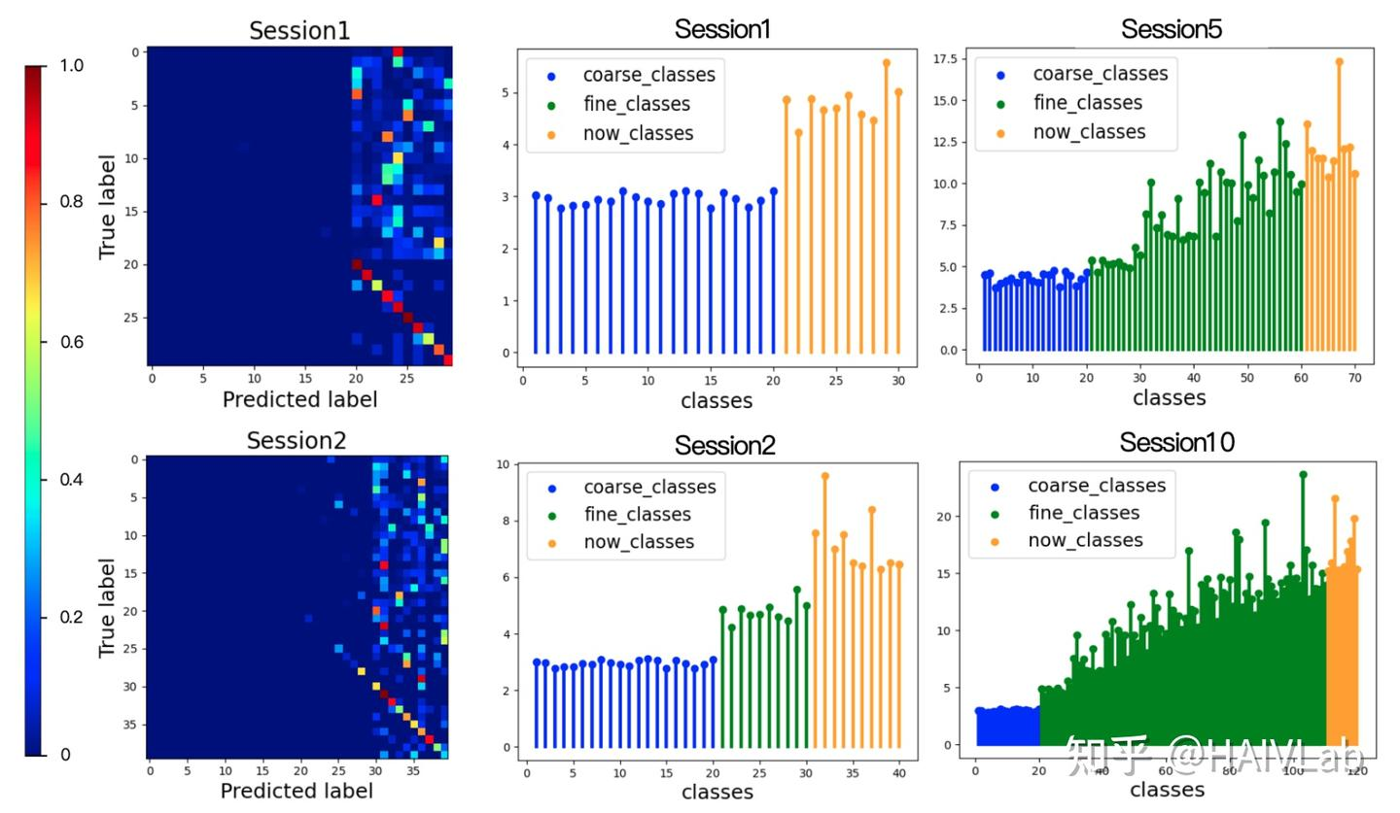
\includegraphics[width=0.82\linewidth,height=0.42\textheight,keepaspectratio]{figures/confusion.png}
\caption*{新类别的分类器权重可能逐渐变大，从而偏向新类别}
\end{figure}

在三个主要基准上进行了实验：

\begin{itemize}
  \item CIFAR-100
  \item BREEDS
  \item tieredImageNet
\end{itemize}

例如，在 BREEDS 的 living17 设置中，Knowe 的平均准确率为 54.62\%，遗忘率为 0.33；在entity30 设置中，平均准确率为 47.79\%，遗忘率为 0.32。

这些结果说明，Knowe 在这类粗到细增量学习任务中，能够比较好地兼顾新类别学习和旧类别保持。

总而言之，除了一个重要的问题 C2FSCIL，Knowe 提出了一种不同的知识组织方式：

\begin{itemize}
  \item 特征空间负责提前学习具有泛化能力的视觉表示；
  \item 分类器权重负责记录已经学到的类别知识；
  \item 增量阶段只需要扩展分类器，而不必反复改变整个模型。
\end{itemize}

这让我们可以在没有旧训练数据的情况下，逐步扩展模型的细粒度识别能力。如同人的知识学习一样，持续学习不是万能的，增量学习不是无所不能的，基础阶段底子也很重要，要对未来有所准备。增量阶段能否学好新知识，不仅取决于增量阶段采用什么学习方法，也取决于初始训练阶段是否为未来的知识扩展做好了准备。

\paragraph{相关工作}

\begin{itemize}
  \item Xiang Xiang*, Yuwen Tan, Qian Wan, Jing Ma, Alan L. Yuille, Gregory D. Hager. Coarse-ToFineIncrementalFew-Shot Learning. In ECCV, 2022.
\end{itemize}

\section{HypKnowe：什么样的特征空间几何表示更适合层次化知识演进？}

\begin{figure}[H]\centering
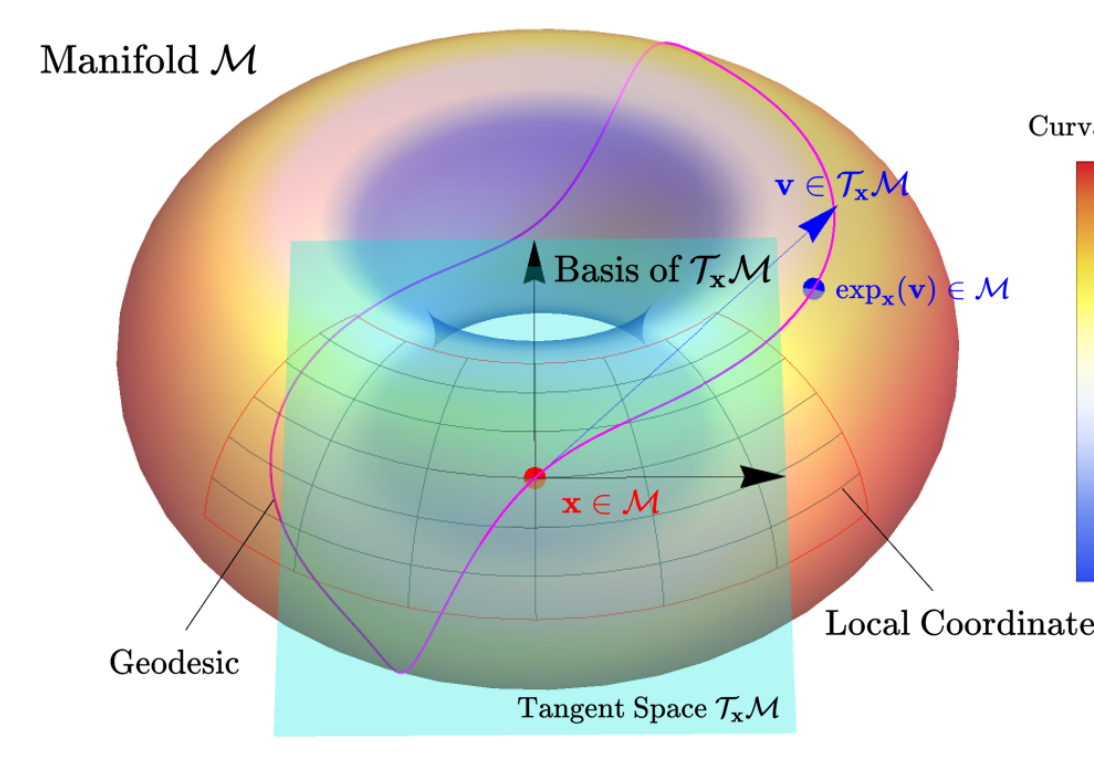
\includegraphics[width=0.82\linewidth,height=0.42\textheight,keepaspectratio]{figures/manifold.png}
\end{figure}

在《C2FSCIL \& Knowe：从类别增量学习走向语义细化》中，Knowe 已经解决了粗到细少样本增量学习中的一部分稳定性问题，从对比学习准备特征空间的有效性出发，我们重新审视特征空间问题，得到的一个自然的问题是：粗粒度类别和细粒度类别本身具有层次结构，是否有一种更适合表达这种层次关系的特征空间？

\begin{figure}[H]\centering
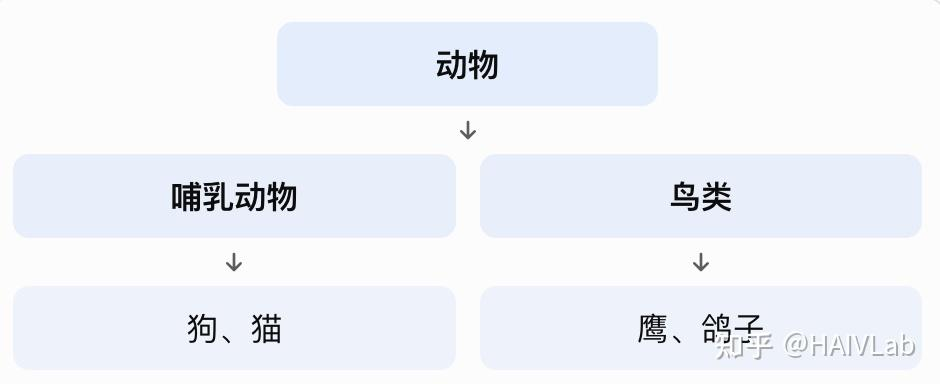
\includegraphics[width=0.82\linewidth,height=0.42\textheight,keepaspectratio]{figures/tree.png}
\caption*{类别天然具有从上层概念到下层细分类别的层次结构}
\end{figure}

Knowe 主要在传统的欧氏空间（Euclidean Space）中进行特征表示。欧氏空间擅长表达一般的几何距离关系。但对于层次结构，如果类别树不断向下扩展，子类别数量可能快速增加。而双曲空间（Hyperbolic Space）具有负曲率，其空间体积随半径增长得非常快，因此能够用相对有限的维度表达丰富的层次关系。直观地说：

\begin{itemize}
  \item 越靠近中心，可以理解为越高层、越抽象的概念；
  \item 越向空间边缘，可以容纳越多细粒度的类别；
  \item 不同分支可以在空间中逐渐展开。
\end{itemize}

因此，双曲空间常被用于知识图谱、层次分类和树状数据表示。既然粗到细学习本身就具有层次结构，那么使用双曲空间可能更符合这个问题的几何特征。HypKnowe （Hyperbolic Knowe）基于 Knowe 的算法框架，将特征映射、对比学习和分类器都调整到双曲几何框架下，尽量保证整个学习过程的几何一致性：

\begin{figure}[H]\centering
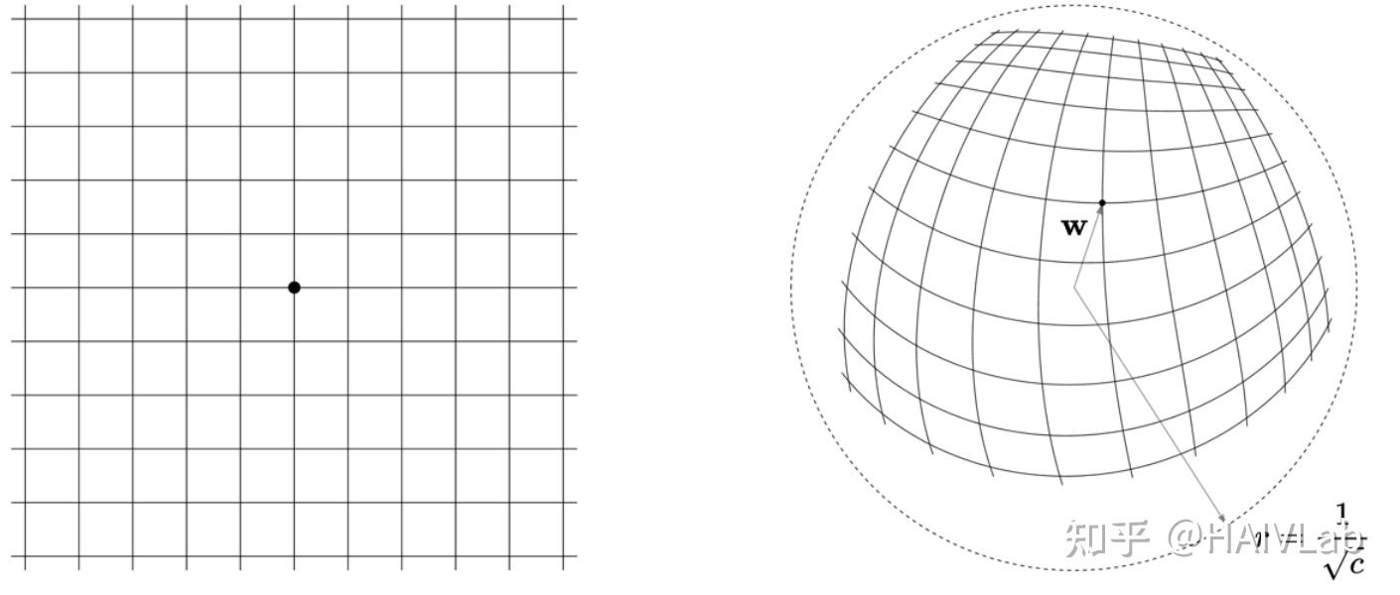
\includegraphics[width=0.82\linewidth,height=0.42\textheight,keepaspectratio]{figures/poincare.png}
\caption*{将欧式特征空间改造成双曲空间}
\end{figure}

①

Hyperbolic

Mapping

Layer

在特征提取网络之后加入双曲映射层，将欧氏特征映射到 Poincaré Ball（庞加莱球）中。②

Hyperbolic

Contrastive

Loss

将原有对比学习中的内积相似度改成基于双曲距离的度量，在双曲空间中学习特征之间的关系。

③

Hyperbolic

Fully

Connected

Layer

将普通全连接分类层改为双曲版本，使分类过程也能够在双曲空间中进行。

除此之外，针对新类别小样本导致过拟合的问题，在双曲空间提出基于概率分布估计的特征增强方法（原来只有少量真实特征，现在根据它们估计一个分布，在这个分布附近生成额外的训练特征）。在三个数据集 CIFAR-100、tieredImageNet、OpenEarthSensing （OES，包含 189 个细粒度类别，并将这些类别组织成 10 个粗粒度类别）上进行了实验：

\begin{table}[H]\centering
\caption*{HypKnowe 平均准确率}
\begin{tabular}{llll}\toprule
\textbf{数据集} & \textbf{Knowe 基础版本平均准确率} & \textbf{加入双曲空间} & \textbf{双曲空间+特征增强} \\ \midrule
CIFAR-100 & 46.406 & 48.875 & 50.528 \\
tieredImageNet & 33.590 & 37.351 & 37.822 \\
OES & 51.066 & 58.848 & 59.084 \\
\bottomrule\end{tabular}
\end{table}

可以看到双曲空间在三个数据集上都提高了平均准确率（在 OES 上，提升尤其明显），遗忘率并没有因为这些改动而明显恶化（在 OES 上，遗忘率从 0.250 降到 0.200）。简言之，Knowe 将特征学习与分类器学习解耦，通过冻结旧类别权重和归一化，平衡稳定性与可塑性，出发点是学习策略——如何在没有旧数据的情况下学习新类别？而HypKnowe 将表示、对比学习和分类过程扩展到双曲空间，更自然地建模类别层次结构，出发点是表示几何——什么样的特征空间更适合表达粗到细的类别关系？更全局一些，Knowe 和 HypKnowe 研究的是类别本身具有层次结构时，如何从粗粒度知识逐渐扩展到细粒度知识。而 SSIAT 和 RAA 研究的则是类别增量过程中，模型内部的表示和参数如何变化，以及如何控制这种变化。所以它们不是完全相同的问题，而是从不同角度研究持续学习中的稳定性与可塑性。

而且，开放世界中的知识变化，不一定表现为完全陌生的新类别，也可能表现为对已有知识的逐步细化。这和一般的 OOD 检测有区别：OOD 检测在于发现输入超出了当前已知类别范围；而 C2FSCIL：当已有类别知识逐渐细化时，如何让模型持续学习。持续学习并不总是意味着不断增加新的类别。有时，模型需要做的是把已经认识的事物理解得更加细致。从“这是一只狗”到“这是一只什么品种的狗”，本质上是已有知识的逐步细化，而不是简单地增加一个互不相关的新类别。

\paragraph{相关工作}

\begin{itemize}
  \item Jiaxin Dai, Xiang Xiang*: Hyperbolic Coarse-to-Fine Few-ShotClass-Incremental Learning. In Conference on Lifelong Learning Agents (CoLLAs), Proceedings of Machine Learning Research, 2026.
\end{itemize}

\section{EHS：预留类别扩展的特征空间}

在《SSIAT：从发现分布偏移，到适应分布偏移》中，我们假设如果一批新图片在模型更新前后整体向某个方向移动了，那么与它们在旧特征空间中比较接近的旧类别的特征中心也可能受到相似方向的影响。基于这一观察，我们利用新类别样本的特征变化，估计旧类别可能发生的语义偏移，并据此调整旧类别的特征中心，使模型在学习新知识的同时，尽可能保留已有知识——新知识到来后，适应已有表示的变化。

但这也让我们进一步思考：既然模型未来还会不断学习新类别，能不能不只是等到新类别出现后再适应，而是在最初训练时就为未来的类别扩展做好准备？例如，模型最初只需要识别 10 个类别，但我们知道，未来还会有更多类别陆续加入。那么，初始训练阶段形成的特征空间，是否应该提前考虑这些新类别的到来——新知识到来之前，如何为未来的类别扩展做好准备？

\begin{figure}[H]\centering
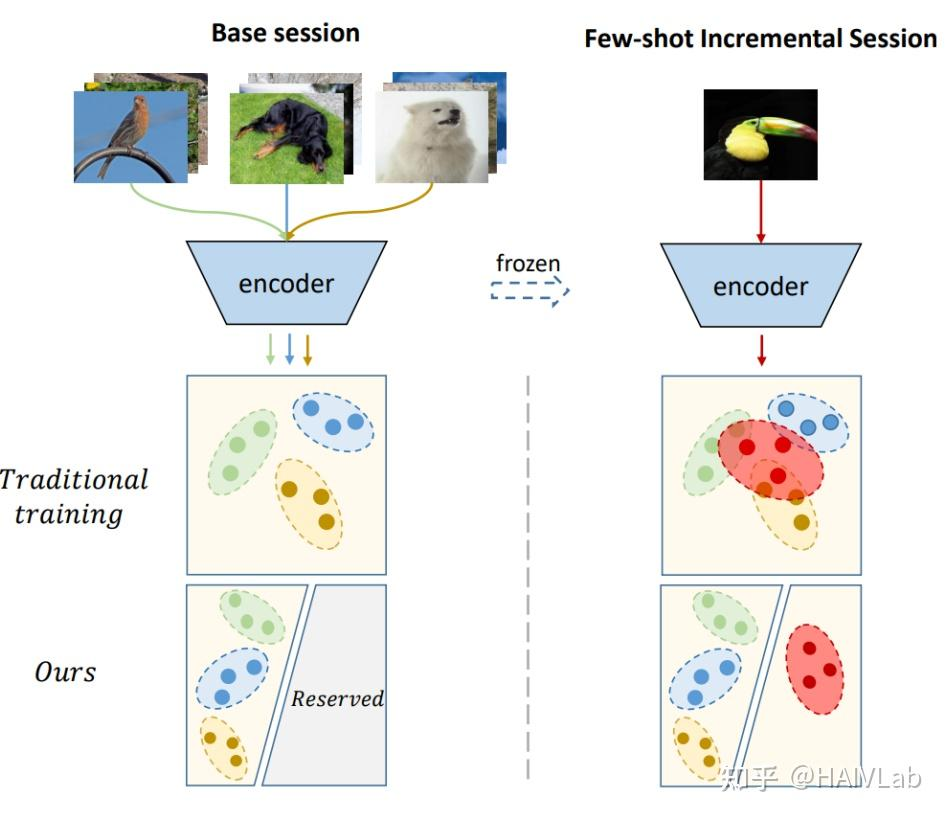
\includegraphics[width=0.82\linewidth,height=0.42\textheight,keepaspectratio]{figures/ehs_base.png}
\caption*{新知识到来之前，如何为未来的类别扩展做好准备——预留特征空间给新类}
\end{figure}

为什么原来的特征空间不够用？特征空间实际上受到激活函数的限制。在很多传统 CNN中，最后的特征提取层使用 ReLU：

\[
\mathrm{ReLU}(x)=\max(0,x)
\]

也就是说，输出永远不会是负数。假设模型提取的是二维特征，ReLU 输出的两个维度都非负，因此特征只能落在第一象限（即使我们把特征归一化到单位圆上，它也只能使用圆的四分之一）。

\begin{figure}[H]\centering
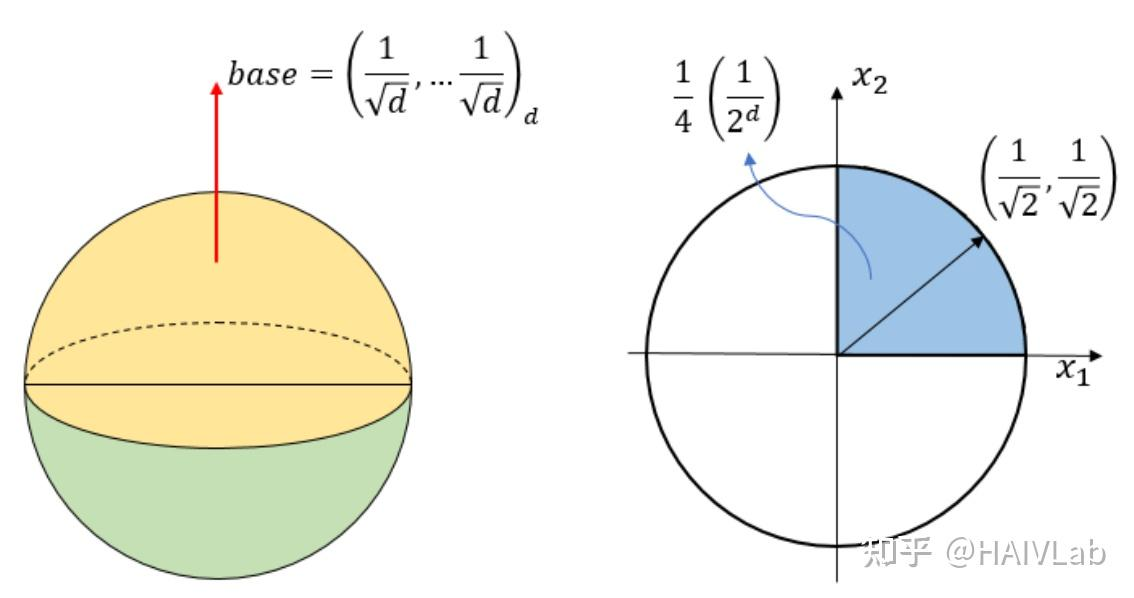
\includegraphics[width=0.82\linewidth,height=0.42\textheight,keepaspectratio]{figures/ehs_sphere.png}
\caption*{Expanding Hyperspherical Space （EHS）的基本想法}
\end{figure}

在 d 维空间中，ReLU 输出只能处于非负正交区域，其对应的超球面区域比例为 $1/2^{d}$。这意味着维度越高，ReLU 所允许的特征方向占整个超球面的比例越小。当然，模型并不是把这个区域完全填满了，而是说它从一开始就受到这样的几何约束。如果未来不断加入新类别，大家都只能在这块有限的区域内寻找自己的位置，特征分布就更容易拥挤、重叠。能不能让特征表示充分利用整个超球空间？从 ReLU 换成 tanh：

\[
\tanh(x)\in[-1,1]
\]

\begin{figure}[H]\centering
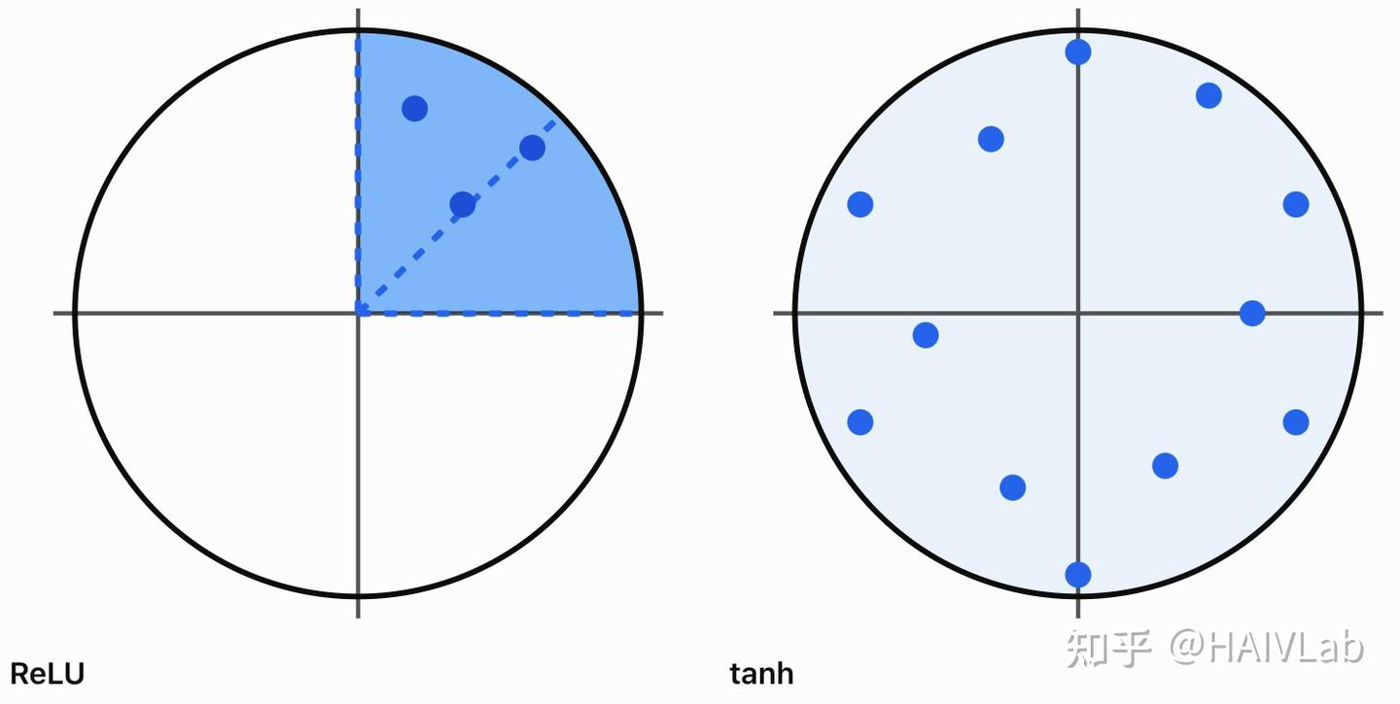
\includegraphics[width=0.82\linewidth,height=0.42\textheight,keepaspectratio]{figures/relu_tanh.png}
\caption*{tanh 正负方向均可使用，覆盖整个圆}
\end{figure}

与 ReLU 不同，tanh 既可以产生正数，也可以产生负数。这意味着特征向量不再被限制在非负区域，可以利用超球面的正负方向。从几何上看，就是让原来只能在一个角落活动的特征，能够分布到整个球面上。这一步的意义并不只是换了一个激活函数，而是改变了模型能够使用的特征空间。不过，仅仅扩大空间还不够。因为如果基础类别和未来类别仍然可以在整个空间里自由分布，那么未来的新类别依然可能与已有类别发生混淆。可以把整个单位超球面想象成一个球，然后从中间切开：上半球分配给当前已经学习的基础类别，下半球预留给未来可能出现的新类别。

未来的新类别还没有出现，怎么知道应该给它们留多少空间？知道未来会有新类别，但在初始训练时，这些类别的真实数据还没有出现。那怎么提前训练模型？可以制造一些假想的未来样本。具体来说，先从两个不同类别中取出图像，经过特征提取网络的中间层，然后把它们的中间特征进行混合，再经过后续网络，得到一个新的伪特征——从两个不同类别的视觉特征中，生成一个介于它们之间的虚拟特征。然后，要求这些伪特征进入下半球。这样，模型在训练基础类别时，不仅把真实的基础类别放到上半球，还利用伪特征对下半球进行约束。相当于提前模拟了一种情况：未来出现了一个新的类别，它的特征应该有自己的活动区域，而不是直接和已有类别混在一起。当然，这些伪特征并不是真正的新类别样本，也不是在训练出未来类别的分类器。它们主要用于塑造特征空间，为未来新类别预留位置。到了增量阶段，由于初始训练阶段已经把基础类别和未来类别的空间分开，新类别的特征就有机会落入预留的下半球。

在 CIFAR-100 和 miniImageNet 上进行实验。

CIFAR-100

FACT：22.50\%

EHS：21.84\%

性能下降减少 0.66 个百分点。

miniImageNet

FACT：22.07\%

EHS：21.76\%

性能下降减少 0.31 个百分点。在消融实验中，单独把 ReLU 换成 tanh，就能降低性能下降。总结一下，训练当前任务时，也要考虑模型未来还需要学习什么。我们不能等到新类别出现时，才发现原来的特征空间已经不够用了。所以，EHS 在初始训练阶段做了三件事：

\begin{enumerate}
  \item 扩大空间：通过 tanh，让特征可以使用完整的超球面。
  \item 划分空间：把基础类别和未来类别安排在不同的半球。
  \item 模拟未来：通过伪特征，提前约束未来类别可能使用的空间。
\end{enumerate}

当然，EHS 预留的是类别扩展的几何空间，并不意味着它已经保留了每个基础类别内部尚未学习的细粒度语义信息。它解决的是“未来出现新类别时，特征空间如何容纳它们”，而不是“未来一个粗粒度类别如何被细化成多个子类别”。

\paragraph{相关工作}

\begin{itemize}
  \item Yao Deng, Xiang Xiang. Expanding Hyperspherical Space for Few-ShotClass-Incremental Learning. In WACV, 2024.
\end{itemize}
